\cotefile{79}
\scanpage{145}
% archive sheet number: 144
% L1–4
ce qui, par la définition de l'opération de $Z'_n$ sur l'une des structures $n$ polygonales sur un ensemble $E$, \deleted{\unsure{à deux élts}}, implique qu'on a un isomorphisme canonique
% L5
\[
p^{-1}(\dot\lambda)\wedge\mu(i)\wedge\mu(\dot\lambda i)\simeq
\underset{\substack{\text{torseur unité}\\\text{sur }\pm1}}{\mathbb{1}}.
\tag*{(43)}
\]
% L6–10
où
\[
 p:\underset{\substack{\Vert\\\Lambda_n^*}}{Z_n}\longrightarrow
 \underset{\substack{\Vert\\\Lambda_n^*/\pm1}}{Z'_n}
\]
\deleted{\unsure{est}} est l'hom. canonique, \deleted{\unsure{surj.}} de degré 2 (\uline{NB} on a \deleted{supposé} $n\ne2$ donc $\deleted{\unsure{+}}1\ne-1$ dans $\Lambda_n$). On a en fait que pour
% L11
\[
\lambda\in p^{-1}(\dot\lambda),\quad \omega\in\mu(i),\quad \omega'\in\mu(i'=\dot\lambda.i)
\]
% L12
on a
\[
\lambda\wedge\omega\wedge\omega'=1\quad\Longleftrightarrow\quad
\omega^{\deleted{\unsure{\lambda}}\,\prime}_E=\omega_E^\lambda
\tag*{(44)}
\]
% L13–15
où $\omega_E,\omega'_E$ sont \deleted{\unsure{interprétées comme} des} permutations circulaires de l'ensemble-étoile $E$ qui correspondent aux orientations $\omega,\omega'$.

% L16–20
A priori l'isomorphisme (43) dépend du choix du sommet $s$. Mais par transport de structure, il est le $=$ pour deux sommets $s,s'$ tels que l'on ait
\[
s'=g.s,\quad\text{avec }g\in G_0^{\unsure{*|+}}
\]
% L21–25
à condition de supposer que $g$, opérant sur $\mu(i)$ et $\mu(\unsure{\lambda'|\dot\lambda i})\unsure{\vphantom{i}^{\epsilon}}$, opère avec le $=$ signe. Si on admet que c'est tjrs le cas (cf plus bas), il suffit de prendre $g\in G_0^+$, \deleted{\unsure{et l'obstruction}}\inserted{\unsure{moy.nt|moy.} une certaine orientation} commune
\[
 G_0\xrightarrow{\mathrm{sg}}\pm1\,,\tag*{(45)}
\]
\scanpage{146}
\mspage{74}
% archive sheet number: 145
% L1–7
et comme $G_0^+$ est transitif sur $S$, il s'ensuit bien que (43) est indépendant du choix de $s\in S$. [Si on ne supposait pas les $P_i$ réguliers, il y aurait lieu soit de mettre un axiome d'indépendance, soit de se fatiguer pour prouver cette indépendance par voie combinatoire, en termes des autres propriétés\ldots] Ceci dit, si $(\lambda,\omega,\omega')\in\Lambda_n\times\mu(i)\times\mu(\dot\lambda.i)$ se correspondent par (44) (pour un $s$, donc pour $\forall\,s$) on posera par définition
% L11–12
\[
\left\{\begin{aligned}
 \omega'&=\lambda.\omega &&(\omega\in\mu(i),\ \omega'\in\mu(i'\unsure{)|\vphantom{)}}=\mu(\dot\lambda.i)\\
 \Longleftrightarrow\quad\omega'_E&=\omega_E^\lambda
 \quad\substack{\text{pour tte étoile}\\\text{(ou une étoile)}}&&\lambda\in\Lambda_n^*).
\end{aligned}\right.
\tag*{(46)}
\]
% L12 left
% slanted
\margin{Il est clair déjà que $\forall\,\omega,\omega'\in\unsure{\vec\Pi|\vec\pi}$, $\exists1\ \lambda\in Z_{\deleted{\unsure{m}}n}=\Lambda_n^*$, avec $\omega'=\lambda.\omega$}
% L13–14
Soit de même $\lambda'\in\Lambda_n^*$, $i''=(\lambda'\lambda\deleted{\unsure{)}})i=\lambda'i'$, considérons $\omega''=\lambda'.\omega'\inserted{\in\mu(i'')}$, caractérisé par
% L15
\[
\omega''_E=(\omega'_E)^{\lambda'}\quad\text{donc}\quad
 \omega''_E=((\omega^{\unsure{*}}_E)^\lambda)^{\lambda'}=(\omega_E)^{\lambda\lambda'}
\]
% L16–17
on a donc aussi, par définition de $(\lambda\lambda').\omega^{*}$, $\omega''=(\lambda\lambda').\omega$ \deleted{\unsure{d'où}}, d'où la relation d'associativité
% L18
\[
\lambda'(\lambda\omega)=(\lambda'\lambda).\omega\,,\tag*{(47)}
\]
% L19–20
donc la loi (46) définit \deleted{bien} une opération du groupe $\Lambda_n^*$ sur $\vec\Pi$, \deleted{que} de sorte que
% L21
\[
\vec\Pi\quad\text{est un torseur sous }\Lambda_n^*\text{ via }(46).\tag*{(48)}
\]
% slanted
\margin{Ceci marche également pour le cas de l'octaèdre !}

% L22
\deleted{\unsure{du groupe|Le groupe}} Essayons de prouver que les conditions
\scanpage{147}
% archive sheet number: 146
% L1–6
d'orientation \deleted{\unsure{$\varepsilon_i$}} $\mathrm{sg}_i$ $(i\in\Pi)$ sur $G_0$ sont les $=$s (cf plus haut). Si $n$ impair, \unsure{cel|cela} provient du fait que sur $G_0$, engendré par des \deleted{\unsure{rel.}}\unsure{gén.} $\tau_0,\tau_1,\tau_\infty$ satisfaisant aux relations (40)(41), il y a \deleted{sous-groupe}\inserted{alors un} unique sous-groupe d'indice 2, de façon plus précise
% L7
\[
 (G_0)_{\rm ab}\simeq \deleted{\unsure{Z}}\pm1 \qquad\text{si }n\text{ impair}
 \tag*{(49)}
\]
% L8–12
$[\![$\uline{NB} \unsure{En tous cas|En tout cas}, $(G_0)_{\rm ab}$ est \deleted{\unsure{eng.}} le groupe abélien engendré par les trois él. d'ordre 2, $\dot\tau_0,\dot\tau_1,\dot\tau_\infty$ \inserted{donc est un quotient de $\mathbb F_2^3$} et $\dot\rho_\infty^3=1$ \deleted{\unsure{se tr}} implique $\dot\rho_\infty=1$ i.e. $\dot\tau_1\dot\tau_0=1$ i.e. $\dot\tau_0=\dot\tau_1$, donc $G_{0\,\rm ab}$ est engendré par $\dot\tau_1,\dot\tau_\infty$, avec la relation
% L13
\[
(\dot\tau_1\dot\tau_\infty)^n=1,\quad\text{i.e. }\dot\tau_1=\dot\tau_\infty\quad\text{si }n\text{ impair}
\tag*{(50)}
\]
% L14–15
ce qui montre notre assertion pour $n$ impair. Pour $n$ pair, on aura
% L16
\[
(G_0)_{\rm ab}\simeq\{\dot\tau_1,\dot\tau_\infty\mid\dot\tau_1^2=\dot\tau_\infty^2=\dot\tau_1\dot\tau_\infty\}\simeq\mathbb F_2\times\mathbb F_2,\tag*{(51)}
\]
% L17–19
il y a donc \inserted{un ens $X$ de} \uline{trois} caractères \deleted{d'ordre} non triviaux $G_0\longrightarrow\pm1$, qui a priori peuvent être permutés entre eux par \inserted{$G$, \deleted{via $G/G_0$} opérant sur $G_{0\,\rm ab}$ via $G/G_0\simeq$}\deleted{\unsure{Z}}\,$Z'_n$. Mais comme $Z\subset G$ centralise $G_0$, $\operatorname{Im}(\underset{\simeq Z'_n}{Z}\mathrel{-}Z'_n)$ (par $\lambda\longmapsto\lambda^2$) opère trivialement, donc $Z'_n$ opère sur $X$ via
% L22–25
$Z'_n/{Z'_n}^2$ \deleted{\unsure{d'ordre}}, dont l'image dans $\unsure{\mathfrak S_X|\mathscr S_X}\simeq\mathfrak S_3$ est donc un 2-groupe \deleted{\unsure{et} on voudrait prouver}\inserted{donc ou bien réduit} à l'élément neutre (et alors on gagne), ou bien une transposition \deleted{et on voudrait que}\inserted{Dans ce dernier cas}, on reste
\scanpage{148}
\mspage{75}
% archive sheet number: 147
% L1–6
que, ou bien les $\chi_i$ sont égaux -- et \inserted{alors} égaux \deleted{\unsure{au}}\inserted{à l'unique} caractère de $X$ laissé fixe par l'action précédente -- ou bien $\chi_i$ prend deux valeurs $\chi,\chi'$, correspondant à \deleted{\unsure{deux}} la partition de $\Pi$ en deux classes suivant le \deleted{\unsure{caractè}} ss-groupe de $Z'_n\simeq Z$ noyau du caractère
% L7
\[
\varepsilon: Z'_n\longrightarrow\{\pm1\}
\]
% L8–15
qui décrit l'action de $Z'_n$ sur $X$. Mais il faudrait déjà se rendre compte s'il peut bien arriver que l'action de $Z'_n$ sur $X$ soit non triviale -- dans le cas congruentiel défini par \deleted{\unsure{$G_0$}} un module libre de rg 2 $M$ sur $\Lambda_n$, le premier cas où la question se pose est pour $n=\deleted{\unsure{8|3|5}}\unsure{5|8}$, $Z'_n\simeq\deleted{\unsure{2}}\pm1$, quelle est son action sur $[\mathrm{Gl}'(2,\mathbb Z/\deleted{\unsure{8|5}}\unsure{5|8}\mathbb Z)^{\pm1}]_{\rm ab}$ ? Tant qu'à faire, autant passer à la limite sur $n$ et se demander : quelle est, \deleted{l'action de relèvement}\inserted{pour la structure d'extension}
% L18
\[
1\longrightarrow \mathrm{Gl}'(2,\widehat{\mathbb Z})^{\pm}
 \longrightarrow\mathrm{Gl}'(2,\widehat{\mathbb Z})
 \mathrel{\unsure{-|\longrightarrow}}\widehat{\mathbb Z}^{*}/\pm1\mathrel{-}1
\tag*{(52)}
\]
% L19–21
l'\deleted{\unsure{structure d'extension}}\inserted{opération correspondante}
\[
\left\{\begin{aligned}
&\text{opération de }\widehat{\mathbb Z}^{*}/\{\pm1\}\text{ sur }
[\mathrm{Gl}'(2,\widehat{\mathbb Z})^{\pm}]_{\rm ab}
 \simeq\underbrace{\mathbb F_2\times\mathbb F_2}_{\text{base }\dot\tau_1,\dot\tau_\infty}\\
&\text{i.e. l'homomorphisme}\\
&\hspace{1em}\widehat{\mathbb Z}^{*}/\{\pm1\}\longrightarrow
\unsure{\mathfrak S|\mathscr S}_{\{\dot\tau_1,\dot\tau_\infty,
 \underbrace{\dot\tau_1\dot\tau_\infty}_{\substack{\deleted{\unsure{\dot\rho_0=\dot\tau_0}}\\
 \unsure{\dot\lambda_0^{-1}=\dot\varepsilon_0|\dot\lambda_0=\dot\varepsilon_0}}}\}}\simeq\mathfrak S_3
\end{aligned}\right.
\tag*{(53)}
\]
% L22–25
\deleted{\unsure{j}}il est clair, en regardant le sous-groupe de $G(2,\widehat{\mathbb Z})$ formé des matrices
\[
\left\{\begin{pmatrix}\lambda&\mu\\0&1\end{pmatrix}\ \bigg|\ 
\lambda\in\widehat{\mathbb Z}^{*},\ \mu\in\widehat{\mathbb Z}\ ,\right.
\]
qui est produit $1/2$-direct de $\widehat{\mathbb Z}^{*}$ \deleted{\unsure{de}} (isom au groupe des $\left(\begin{smallmatrix}\lambda&0\\0&1\end{smallmatrix}\right)$
\scanpage{149}
% archive sheet number: 148
% L1–4
et $\widehat{\mathbb Z}.\dot\varepsilon_0$ (isom. au groupe des $\left(\begin{smallmatrix}1&\mu\\0&1\end{smallmatrix}\right)$) que l'action de $\widehat{\mathbb Z}^{*}$ sur $\dot\varepsilon_0$ est bien triviale -- ce qui était clair a priori -- donc l'action de $\widehat{\mathbb Z}^{*}/\pm1$ dans (53) s'exprime par un caractère
% L5
\[
\varepsilon:\widehat{\mathbb Z}^{*}/\pm1\longrightarrow\{\pm1\}\deleted{\unsure{\varepsilon_i}}
\tag*{(54)}
\]
% L6–9
qu'il faudrait expliciter, exprimant de quelle façon un élément arbitraire \deleted{\unsure{de}} $\dot\lambda\in\widehat{\mathbb Z}^{*}/\pm1$ opère sur $\{\underset{\substack{\Vert\\\dot\tau_0}}{\dot\tau_1},\dot\tau_\infty\}$, \deleted{-- rappelons-nous à ce propos que}
% L10
\[
\deleted{r_0=\begin{pmatrix}0&1\\1&0\end{pmatrix},\quad
 r_1=\begin{pmatrix}-1&1\\0&1\end{pmatrix},\quad
 r_\infty=\begin{pmatrix}-1&0\\0&1\end{pmatrix}.}\tag*{\deleted{(55)}}
\]
% L11–17
\deleted{Si $\varepsilon$ n'est pas le caractère trivial,}

\deleted{la structure connue de $\widehat{\mathbb Z}^{*}$ montre qu'il suffit de tester la valeur de $\varepsilon$ pour les $\mathbb Z/n\mathbb Z$}

\deleted{A vrai dire, il est clair a priori que \deleted{la valeur} $\varepsilon$ est trivial sur les $\mathbb Z_\ell^{*}\simeq\mathbb Z_\ell\times\mathbb F_\ell^{*}$ avec $\ell$ nb premiers impairs [car il est trivial, sur $\mathbb Z_\ell$ la composante $\mathbb Z_\ell$, ce qui montre qu'il suffit de regarder}
% L18–19
\deleted{Écrivons}
\[
\deleted{\widehat{\mathbb Z}^{*}\simeq\widehat{\mathbb Z}_2^{*}\times
\underbrace{\widehat{\mathbb Z}^{*\,\prime}}_{\displaystyle
\prod_{\substack{\ell\text{ premier}\\\text{impair}}}\mathbb Z_\ell^{*}}\, ,}
\]
% L20–24
\deleted{il est clair que si $\varepsilon\ne1$, alors $\varepsilon$ ne provient \uline{pas} d'un caractère sur le facteur $\widehat{\mathbb Z}^{*\,\prime}$ (i.e. il ne provient pas d'un caractère sur $(\mathbb Z/n\mathbb Z)^{*}$ avec $n$ \deleted{premier} impair), donc dans ce cas la composante du caractère suivant $\widehat{\mathbb Z}_2^{*}$}
\scanpage{150}
\mspage{76}
% archive sheet number: 149
% L1
\deleted{est non triviale. Donc pour voir si}

% L2–5
Notons que l'on obtient déjà la valeur ``universelle'' de $(\mathrm{Gl}'_{\deleted{\unsure{n}}}(2,\mathbb Z/n\mathbb Z)^{\pm})_{\rm ab}$, \inserted{savoir $\mathbb F_2\times\mathbb F_2$,} pour $n=4$, de telle façon qu'il est quand $=$ évident a priori que $\varepsilon$ se factorise par
% L6
\[
\widehat{\mathbb Z}^{*}/\pm1\mathrel{\unsure{-|\longrightarrow}}
\underbrace{(\deleted{\unsure{\widehat Z}}\mathbb Z/\deleted{\unsure{8}}4\mathbb Z)^{*}/\pm1}_{\substack{\deleted{\unsure{\pm1\simeq Z'_8}}\\Z'_4=\{1\}}}
\longrightarrow\{\pm1\}\,,
\tag*{\deleted{(\unsure{55|56})}}
\]
% L7–11
\deleted{et la seule question est si ce caractère est ou non trivial, i.e. si $(\mathbb Z/8\mathbb Z)^{*}/\pm1$ \inserted{$\simeq\pm1$} opère trivialement, ou non, sur $(\mathrm{Gl}'(2,\mathbb Z/8\mathbb Z)^{\pm})_{\rm ab}\simeq\mathbb F_2\times\mathbb F_2$.}

\deleted{Notons que $\mathrm{Gl}'(2,\mathbb Z/4\mathbb Z)^{\pm}\simeq\unsure{\mathfrak S_4|\mathscr S_4}\times\pm1$.}
% L12
ce qui montre que \uline{le caractère $\varepsilon$ est trivial !}$]\!]$

% L13–17
\deleted{\unsure{Reven|Revenons}} Notons que \inserted{\unsure{si $n$|si on}} $G_0^+=\mathrm{Aut}^+(S,F_{i_0})$ est le seul sous-groupe d'indice 2 de $G_0$ qui contienne $\rho_0$ (\uline{NB} $\dot\rho_0$ \deleted{\unsure{$=\dot r_0\dot r_\infty$}} $\dot r_1\dot r_\infty$) \deleted{\unsure{et}}\inserted{-- où $\rho_0$ est l'opération de rotation autour d'un sommet déterminé $\deleted{\unsure{a}}s_0\in S$, associée au repère \unsure{$(a_0,s_0,s'_0)$|$(s_0,s_1,s_\infty)$}}, pour prouver que \deleted{\unsure{il est}} $G_0^+$ égal à $G_1^+=\mathrm{Aut}^+(S,F_{i_1})$, pour $i_1=\lambda.i_0$, il suffit de voir que l'on a
% L18
\[
\rho_0\overset{\mathrm{déf}}{=}\rho_{s_0,A_0}\in G_1^+=\mathrm{Aut}^+(S,F_i)\,,
\tag*{(55)}
\]
% L19–20
pour ceci considérons l'étoile
\[
E=\mathrm{Et}_0(s_0)=\mathrm{Et}_1(\dot\lambda.s_0)
\]
% L21–25
$\rho_0$ applique $E$ dans lui-$=$, et est un automorphisme direct \inserted{i.e. une ``rotation''} pour la structure polygonale $A_{0E}=A_0\cap\unsure{\mathcal P_2|P_2}(E)$, \deleted{\unsure{On en devrait aussitôt}}\deleted{\unsure{i.e. appartient à}} On en conclut qu'il est aussi direct pour la structure polygonale $A_{1E}=A_1\cap\mathcal P_2(E)$, puisque $A_{1E}=A_{0E}^{(\dot\lambda)}$ -- donc
\scanpage{151}
% archive sheet number: 150
% L1–5
$\rho_0$, qui fixe $\lambda s_0$ (puisqu'il fixe $s_0$ et commute à $\lambda$) et induit un autom direct de l'étoile de $\lambda s_0$ \deleted{\unsure{pour}} pour $P_1$, est un automorphisme direct pour $P_1$ i.e. on a (54), ce qui achève de prouver
% L6–10
\[
\begin{aligned}
&\text{\deleted{\unsure{les}} les caractères d'orientation \inserted{sur $G_0$} pour les structures}\\
&\text{de polyèdres }P_i\quad(i\in\Pi)\text{ sont les $=$s, i.e.}\\
&\text{il existe un (unique) sous-groupe }G_0^+\text{ de}\\
&G_0,\text{ tel que l'on ait}\\
&\qquad G_0^+=\mathrm{Aut}^+(\unsure{P_i|\Phi_i})\qquad\forall i\in\Pi\ .
\end{aligned}
\tag*{(56)}
\]
% L11
Cela achève en même temps de prouver (48.).

% L12–16
Considérons maintenant l'action (par transport de structure) de $G=\mathrm{Aut}(S,F)$ sur $\unsure{\vec\Pi|\vec\pi}$, il est immédiat que cette action \deleted{\unsure{commute}}\inserted{respecte} la \deleted{\unsure{celle de}} structure de $\Lambda_n^*$-torseur sur $\vec\Pi$, d'où on déduit un unique homomorphisme
% L17
\[
G\xrightarrow{\chi}(\mathbb Z/n\mathbb Z)^*\qquad
\text{le ``\uline{caractère}}\quad\substack{\strut\\\text{\uline{\unsure{cyclotomique|cyclotromique}}''}}
\tag*{(57)}
\]
% L18–19
caractérisé par la propriété
\[
\forall\,\underbrace{i\in\Pi,\ \omega\in\mu(i)}_{\text{d'où }\alpha=(i,\omega)\in\vec\Pi},
\ \inserted{g\in G,}\ \text{on a}\quad
\underbrace{g\overbrace{(i,\unsure{\omega|\lambda})}^{\alpha\in\vec\Pi}}_{\substack{\text{transport}\\\text{de structure}}}
=\underbrace{\chi(g).\overbrace{(i,\omega)}^\alpha}_{\substack{\text{opération}\\\text{arithmétique}\\\text{d'exposant}\\
\chi(g)\text{ sur la}\\\text{structure}\\P_i=(S,A_i,F_i)}}.
\tag*{(58)}
\]

% L20–22
Le caractère $\chi$ factorise le caractère $\chi':G\longrightarrow(\mathbb Z/n\mathbb Z)^*/\pm1\deleted{\unsure{\simeq Z_n}}=Z'_n\simeq Z$ (``\uline{caractère demi-cyclotomique}''), i.e. on a commutativité \unsure{du|de|dans}
\scanpage{152}
\mspage{77}
% archive sheet number: 151
% L1–2
\diagram{\[
\begin{tikzcd}[ampersand replacement=\&]
G \arrow[r,"\chi"] \arrow[dr,"\chi'"'] \& (\mathbb Z/n\mathbb Z)^* \arrow[d,"\mathrm{can.}"]\\
\& Z\simeq(\mathbb Z/n\mathbb Z)^*/\pm1\ .
\end{tikzcd}\tag*{(59)}
\]}
% L3–5
On voit que le noyau de $\chi$ est $G_0^+$, de sorte que la suite exacte (17) peut aussi se déduire d'une suite exacte
% L6–7
\diagram{\[
\begin{tikzcd}[ampersand replacement=\&,column sep=1.3em]
1 \arrow[r] \& G_0^+ \arrow[r,dash] \& G \arrow[r,"\chi","\text{car. cyclotomique}"'] \& (\mathbb Z/n\mathbb Z)^* \arrow[r] \& 1\ .\\
\& \& Z\simeq(\mathbb Z/n\mathbb Z)^*/\pm1 \arrow[u,hook] \arrow[ur,maps to,"\dot\lambda\mapsto\lambda^2"'] \& \&
\end{tikzcd}\tag*{(60)}
\]}
% slanted
\margin{sauf dans cas octaédral ($n=4$) où il faut remplacer $Z$ par $\{1\}$}
% L8–10
\deleted{\uline{NB} On lit} par
\[
\begin{aligned}
G_0&=\{g\in G\mid\chi(g)\in\{\pm1\}\}\\
&[=\operatorname{Ker}(\chi':G\longrightarrow(\mathbb Z/n\mathbb Z)^*/\pm1\ ]
\end{aligned}\tag*{(61)}
\]

% L11–12
\uline{NB} On lit sur (60) que
\[
\underbrace{Z\cap G_0^+}_{=\mathrm{Cent}(G_0^+)}=
({}_2(\mathbb Z/n\mathbb Z)^*)/(\pm1)\simeq\mathbb F_2^{\mathbb P(n)'}/\mathrm{diag}
\tag*{(62)}
\]
% slanted
\margin{y compris cas $n\deleted{\unsure{\ne}}=4$, \deleted{Dans le cas $n=4$} où \deleted{\unsure{$Z$ est de}} on trouve \deleted{\unsure{où}} $\underbrace{Z}_{\{1,\unsure{a|0}\}}\cap G_0^+=\{1\}$}
% L13–16
$\mathbb P(n)$ est l'ensemble des nbs premiers \deleted{impairs} qui divisent $n$, et $\mathbb P'(n)$ est égal à $\mathbb P^{\deleted{\unsure{*}}}(n)$ sauf si $2\in\mathbb P(n)$ et si 2 intervient avec un \deleted{\unsure{fact}} exposant \inserted{$e_2$} $\ne2$ \deleted{i.e. sauf si $\left\{\begin{smallmatrix}n\equiv0\ (2)\\ n\not\equiv0\ (4)\end{smallmatrix}\right.$, auquel cas} auquel cas on pose
% L17–19
\[
\left\{\begin{aligned}
\mathbb P'(n)&=\mathbb P(n)\setminus\{2\}&&\text{si }e_2=1\\
\mathbb P'(n)&=\mathbb P(n)\amalg\{\substack{\text{un élément}\\\text{supplém.}}\}&&\text{si }e_2\ge3\\
(\mathbb P'(n)&=\mathbb P(n)&&\text{si }e_2\in\{0,2\}
\end{aligned}\right.\tag*{(63)}
\]
% L20–21
donc
\[
Z\cap G_0^+\simeq\mathbb F_2^\nu\quad\text{avec }\nu=
\underbrace{\nu(n)}_{\substack{\text{nb de facteurs}\\\text{premiers de }n}}
\unsure{-|+}1+\varepsilon,\quad\varepsilon=
\begin{cases}
\unsure{0}\ \deleted{\unsure{\text{si}}}\ e_2\in\{0,\unsure{2|1}\}\\
-1\ \text{si }e_2=1\\
+1\ \text{si }e_2\ge3
\end{cases}.
\tag*{(64)}
\]
\scanpage{153}
% archive sheet number: 152
% L1–4
Notons que
\[
\nu\ge\nu(n)-2,\ 0
\]
ce qui implique qu'on ne peut avoir $\nu=0$ i.e. $G_0^+\cap Z$ que dans les cas disjoints \(\substack{\nu(n)=2,\ n=2p\ldots\\\nu(n)=1\ \text{avec}\ldots}\)
% L5–7
\[
G_0^+\cap Z=0\quad\Longleftrightarrow\quad
\left\{\begin{aligned}
&\left.\begin{aligned}
 n&=2p^e\quad p\text{ premier impair}\\
 n&=p^e\quad p\text{ premier impair}
 \end{aligned}\right|e\ge1\\
&n=\deleted{\unsure{2^e}}4\quad\deleted{\text{\unsure{ou}}}\ (\text{cas \unsure{octaédral|octaèdral}})
\end{aligned}\right.
\tag*{(65)}
\]
\deleted{Mais on fait attention qu'ici, dans le cas où}

% L8–9
Dans le cas $n=2^{\deleted{\unsure{a}}e}$ avec $e\ge3$, on trouve \deleted{$G^+\cap Z\simeq\mathbb F_2$.}
\[
 {}_2Z\simeq\mathbb F_2^2,\qquad G_0^+\cap Z\simeq\mathbb F_2
 \qquad(\text{pour }n=2^e,e\ge3).
\tag*{(65)}
\]

% L10–11
On va encore \deleted{définir}\inserted{introduire} l'application canonique
\[
\vec F\xrightarrow{\vec\tau_F}\deleted{\unsure{(\mathbb Z/n\mathbb Z)^*}}\unsure{\vec\Pi|\vec\pi}
\tag*{(66)}
\]
% L12–15
\unsure{s'inscrivant|s'insérant} dans le diagramme commutatif \inserted{(en fait un carré cartésien)}
\diagram{\[
\begin{tikzcd}[ampersand replacement=\&]
\vec F \arrow[r,"\vec\tau_F"] \arrow[d,"\mathrm{can}"'] \arrow[dr,phantom,"\text{\uline{cart}}"] \& \vec\Pi \arrow[d,"\mathrm{can}"]\\
F\arrow[r,"\tau_F"'] \& \Pi
\end{tikzcd}\tag*{(67)}
\]}
(cf (24) pour le ``type'' des faces)
% L16–21
en notant que toute face \deleted{\unsure{orientée}} \deleted{\unsure{définit $(f,\omega)$|$\tau_F(f,\omega)$}}, $f\in F$, si $i=\tau_F(f)$ est son type, il y a corresp 1-1 entre l'ens $\unsure{\underline\omega_f|\simeq_f|\vec F_f}$ des deux orientations de $f$, et l'ens $\mu(i)$ des deux \unsure{orientations|orientables} de $P_i$ i.e. des deux éléments de $\vec\Pi$ au dessus de $i$. On trouve de $=$ un diagramme commutatif \inserted{cartésien}
% L22–23
\diagram{\[
\begin{tikzcd}[ampersand replacement=\&]
\vec A \arrow[r,"\vec\tau_A"] \arrow[d,"\mathrm{can}"'] \& \vec\Pi\arrow[d,"\mathrm{can}"]\\
A\arrow[r,dash,"\tau_A"'] \& \Pi\ ,
\end{tikzcd}\tag*{(68)}
\]}
\scanpage{154}
\mspage{78}
% archive sheet number: 153
% L1–3
avec la compatibilité entre (67) (68) :
\[
\begin{aligned}
&\text{si }\vec a\in\vec A\text{ est incidente (\uline{avec orientations induites})}\\
&\text{à }\vec f\in\vec F,\quad\text{alors }\vec\tau_A(\vec a)=\vec\tau_F(\vec f)
\end{aligned}\tag*{(69)}
\]
% L4–8
en d'autres termes on a commutativité dans
\diagram{\[
\begin{tikzcd}[ampersand replacement=\&]
\&\mathrm{Rep}(S,F)\arrow[dl,"\mathrm{can}"']\arrow[dr,"\mathrm{can}"]\&\\
\vec A\arrow[dr,"\vec\tau_A"']\&\&\vec F\arrow[dl,"\vec\tau_F"]\\
\&\unsure{\vec\Pi|\vec\pi}\&\ .
\end{tikzcd}\tag*{(70)}
\]}

% L9–13
Je voudrais maintenant dévisser un peu plus la situation du diagramme (60). Fixons nous un $s_0\in S$, et considérons son stabilisateur \deleted{dans} $G_{s_0}$ dans $G$, on a donc, \margin{\unsure{dévissant|divisant}}
\[
1\mathrel{\unsure{-|\longrightarrow}}\underset{\substack{\wr\Vert\ \text{non canoniquement}\\\mathbb Z/n\mathbb Z}}{G^+_{0s_0}}
 \longrightarrow G_{s_0}\longrightarrow(\mathbb Z/n\mathbb Z)^*
\]
% L14–17
je dis que $G_{s_0}\mathrel{\overset{\chi\mid G_{s_0}}{\unsure{-|\longrightarrow}}}(\mathbb Z/n\mathbb Z)^*$ est épi -- c'est formel, à partir du fait que $G_0^+$ est transitif sur l'ensemble $S$, donc on a une structure d'extension canonique :
% L18–19
\[
1\longrightarrow\underset{\substack{\wr\Vert\\\mathbb Z/n\mathbb Z\ \text{\uline{non} can.}}}{G^+_{0s_0}}
\longrightarrow G_{s_0}\longrightarrow(\mathbb Z/n\mathbb Z)^*\longrightarrow1\ .
\tag*{(71)}
\]
% slanted
\margin{On a envie de noter ce groupe $U_{s_0}$ (``\unsure{unipotent|unipotents}'' !)}
% slanted
\margin{on a envie de le noter $B'_{\unsure{s_0}}$ (``Borel'') / mais il lui manque encore un facteur $G_m$ pour le mériter\ldots}
\scanpage{155}
% archive sheet number: 154
% L1–2
On aimerait scinder cette extension. \deleted{Notons}\inserted{Posons}
\[
\mathrm{Et}_F(s_0)\overset{\mathrm{def}}{=}\coprod_{i\in\Pi}\mathrm{Et}_i(s_0)
=\{s\in S\mid\{s_0,s\}\in A_0\}\,,
\tag*{(72)}
\]
% L3–4
et notons
\[
\deleted{\unsure{G\ \text{est}}}\ G_{s_0}\text{ est transitif sur }\mathrm{Et}_F(s_0)
\tag*{(73)}
\]
% L5–10
ce qui résulte encore formellement du fait que $G$ est transitif sur $\vec A$, \deleted{et $G_0^+$ est transitif sur} le stabilisateur \inserted{dans $G_{s_0}$} d'un élément $t_0\in\mathrm{Et}_F(s_0)$, i.e. le stabilisateur dans $G$ de $a\ (s_0,t_0)\in\vec A$, est un sous-groupe d'ordre 2, contenu dans $G_0^+$ \deleted{\unsure{donc dans}}, de ``déterminant'' égal à $-1$. Son élément non trivial mérite la notation $\tau_\infty$, plus précisément $\tau_\infty^{a_0}$ où $a_0=\{s_0,t_0\}$, égal à $\tau_\infty^{r_0}$ où $r_0$ est un repère de la forme
% L14
\[
r_0=(s_0,t_0,u_0)\ .
\]

% L15–17
Notons que le groupe
\[
Z\simeq(\mathbb Z/n\mathbb Z)^*
\]
opère \uline{librement} sur $S$ (puisqu'il opère par autom d'une structure d'espace homogène), soit $D_t$ \deleted{\unsure{soit}} l'orbite \deleted{\unsure{sous}} d'un $t\in S$. Notons que $Z$ stabilise $\mathrm{Et}_F(s_0)$ (pour tt $s_0\in S$), donc toute orbite \inserted{de $Z$ (un ``\uline{rayon}'')} qui rencontre $\mathrm{Et}_F(s_0)$, est contenue dedans. Choisissons donc, en plus de $s_0\in S$, un rayon \deleted{\unsure{$D$}}
% L23–24
\[
D_0\deleted{\unsure{=Z.t_0}}\subset\mathrm{Et}_F(s_0)\ ,\qquad D_0\ \inserted{Z\text{-}}\text{orbite d'un }
t_0\in\mathrm{Et}_F(s_0)
\tag*{(74)}
\]
\scanpage{156}
\mspage{79}
% archive sheet number: 155
% L1–3
Soit
\[
\begin{aligned}
 T=T_{D_0}&=\text{stabilisateur de }D_0\text{ dans }G_{s_0}\\
 &=\{g\in G_{s_0}\mid\underset{\text{i.e. }g(t_0)\in D_0}{g(D_0)=D_0}\}
\end{aligned}\tag*{(75)}
\]
% L4–6
\deleted{Posons} On a donc
\diagram{\[
\begin{tikzcd}[ampersand replacement=\&,row sep=0.5em,column sep=0.4em]
G^+_{0s_0}=\deleted{\unsure{T|\mathcal U}}U_{\deleted{\unsure{s_0}}}\subset \& G_{s_0} \& =\overset{\deleted{\unsure{B}}}{B'}\\
\& T_{\deleted{\unsure{0}}}\arrow[u,phantom,"\rotatebox{90}{$\subset$}" description] \& ,
\end{tikzcd}
\]}
% L7–8
\deleted{quel est $T\cap G_0^+$} je dis que
\[
T\cap G_0^+=\{1\},\qquad T\xrightarrow{\chi\mid T}(\mathbb Z/n\mathbb Z)^*
\quad\text{épi donc iso}\ \deleted{\unsure{,}}
\tag*{(76)}
\]
% L9–11
en d'autres termes, je dis que $T$ définit un \uline{scindage} de la structure d'ext. (71)
\[
G_{s_0}\simeq\deleted{\unsure{G_{s_0}}}
\underbrace{U}_{G^+_{0s_0}\simeq\underbrace{\mathbb Z/n\mathbb Z}_{\text{non can.}\unsure{^{\mathrm t}|!}}}.
\underset{\substack{\wr\Vert\\(\mathbb Z/n\mathbb Z)^*}}{T}\quad 1/2\ \text{direct}\ .
\tag*{(77)}
\]
% L12–14
Soit donc $g\in G^+_{0s_0}$ qui soit dans $T$ i.e. tel que $g(t_0)\in D_0$ donc $g(t_0)=\dot\lambda t_0$ ($\dot\lambda\in Z$), \deleted{comme $g\in G_0$ et $g$ fixe $s_0$, \unsure{on voit} il s'ensuit que $\{s_0,t_0\}$ et $\{gs_0=s_0,g(t_0)\}$ appartiennent à la $=$ structure $P_{i_0}$ ($i_0\in\Pi$), mais $g(t_0)=\dot\lambda t_0$ \deleted{signifie}\inserted{implique} que} Soit
% L17
\[
i_0=\tau_A(\{s_0,t_0\}),\quad i_1=\tau_A(\{\underset{\substack{\Vert\\g(s_0)}}{s_0},g(t_0)\})
\]
% L18–21
comme on a $g\in G_0$ et $g(s_0)=s_0$, on a donc
\[
i_1=g(i_0)=i_0
\]
et comme $g(t_0)=\lambda.t_0$, on a
\[
i_1=T_\lambda.i_0\qquad\text{d'où}\quad \lambda=1,\quad\text{i.e. }g(t_0)=t_0
\]
% L22–24
\deleted{[on aurait pu dégager : deux points différents d'un rayon, \deleted{\unsure{reliés}} \inserted{$A$-adjacents} à un même $s$, donnent}
\figure{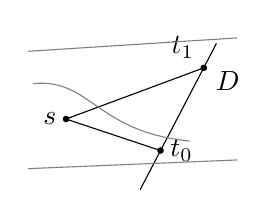
\begin{tikzpicture}[x=1cm,y=1cm,baseline]
\coordinate (s) at (0,0);\coordinate (tzero) at (1.2,-.4);\coordinate (tone) at (1.75,.65);
\draw (s)--(tone) (s)--(tzero) (.94,-.9)--(1.91,.96);
\fill (s) circle (1.2pt) node[left] {$s$};
\fill (tone) circle (1.2pt) node[above left] {$t_1$};
\fill (tzero) circle (1.2pt) node[right] {$t_0$};
\node[right] at (1.78,.48) {$D$};
\draw[gray] (-.48,.86)--(2.17,1.03) (-.48,-.63)--(2.17,-.52);
\draw[gray] (-.42,.45) .. controls (.32,.52) and (.37,-.16) .. (1.57,-.28);
\end{tikzpicture}}
\scanpage{157}
% archive sheet number: 156
% L1–6
[On pourrait dégager
\[
\begin{aligned}
&\text{Soit }s_0\in S,\ D\text{ un rayon. Alors si un \deleted{\unsure{pt}} }t_0\in D\text{ est}\\
&A\text{-adjacent à }s_0,\text{ tous les }t\in D\text{ le sont. L'application}\\
&\qquad D\longrightarrow\Pi\\
&\qquad t\longmapsto\tau_A(\{s_0,t\})\\
&\text{est \uline{bijective}.}\qquad]
\end{aligned}\tag*{(78)}
\]
% L7–10
Ainsi $g\in G_0$ fixe $s_0$ et $t_0$, qui sont adjacents, donc si on avait $g\ne\mathrm{id}$, on aurait $g=\tau_\infty^{\{s_0,t_0\}}$, or $\chi(\tau_\infty)=-1$ \deleted{et} tandis que \deleted{\unsure{$g$}} l'on a supposé $g\in G_0^+$ i.e. $\chi(g)=1$, donc on doit avoir $g=1$.

% L11–13
Prouvons enfin $T\xrightarrow{\chi\mid T}(\mathbb Z/n\mathbb Z)^*=Z$ surjectif. Soit $\lambda^{\unsure{*|\cdot}}\in(\mathbb Z/n\mathbb Z)^*$ \inserted{et soit $\dot\lambda$ son image dans $Z=(\mathbb Z/n\mathbb Z)^*/\pm1$,} alors $\exists\, g\in G_{s_0}$ tel que l'on ait
\[
g\,t_0=\dot\lambda.t_0\tag*{\deleted{(\unsure{74})}\ \unsure{(\ast)|\ast|\text{ou}}}
\]
% L14–17
puisque $G_{s_0}$ est transitif sur $\mathrm{Et}_F(s_0)$, et \unsure{cel|cela} implique que $g\in T$ (75). \deleted{\unsure{A}} La relation $(\ast)$ signifie aussi
\[
\chi'(g)=\dot\lambda\ ,\quad\text{i.e.}\quad\chi(g)\in\pm\lambda\,,
\]
% L18–22
mais d'autre part il y a ambiguïté dans le choix de $g$, via la possibilité
\[
g\longmapsto \deleted{\unsure{\tau}}g\circ\tau_\infty,\qquad\text{donc}\quad\chi(g)\longmapsto\chi(g)\chi(\tau_\infty)
\]
or
\[
\chi(\tau_\infty)=-1
\]
donc en corrigeant au besoin $g$, on gagne !

% L23–27
\uline{Remarque.} Cette façon de trouver une décomposition de $G_{s_0}$ en produit $1/2$ direct $G^+_{0s_0}.\deleted{\unsure{Z}}T_{\unsure{\prime|\,}}$, où $T\subset G_{s_0}$ est tel que $T\longrightarrow\widetilde Z=G/G_0^+$, est ``formelle'' à partir des seuls axiomes $T_0\,1,\ T_0\,4$, et l'axiome de régularité et d'orientabilité $(T_0\,8)$,
\scanpage{158}
\mspage{80}
% archive sheet number: 157
% L1–4
à l'exclusion des axiomes ``arithmétiques'' $T_0\,5)$ $T_0\,6)$ $T_0\,7)$, permettant entre autres d'identifier $\widetilde Z:(\mathbb Z/n\mathbb Z)^*$, et d'interpréter l'action de $Z\simeq Z'_n$ sur $(S,F)$ par voie ``arithmétique''.

% L5–9
Dans cet esprit, partons de la situation suivante : un 2-polyèdre triangulé connexe régulier $P_0=(S,A_0,F_0)$, avec groupe d'autom. $G_0$, et un sous-groupe $Z$ \uline{donné d'avance}
% slanted
\margin{Cette présentation pourrait se développer pour commencer en \unsure{terme|termes} de structures de \uline{graphes}, et indépendamment de toute condition de \uline{régularité}.}
\[
Z\subset\unsure{\mathfrak S_S|\mathscr S_S},\qquad Z\subset\mathrm{Com}_{\mathfrak S_S}(G_0),\ \deleted{\unsure{s}}
\]
% L10–13
satisfaisant la condition supplémentaire (peut. être tjrs vérifiée,\unsure{?} \deleted{\unsure{par}} la condition draconienne de régularité)
\[
\begin{aligned}
&\forall\,\deleted{\unsure{g}}\lambda\in Z,\ \exists f\in\mathfrak S_S\ \inserted{\text{\uline{centralisant }$Z$}}\ \text{telle que }\forall s,t\in S,\ \text{on ait}\\
&(s,t)\in A_0\quad\Longleftrightarrow\quad\{f^{-1}s,f^{-1}\lambda t\}\in A_0
\end{aligned}\tag*{(79)}
\]
% slanted
\margin{cette condition implique que $Z$ est commutatif}
% L14
(cf transcription pp 66$'$ (8)).

% L15–20
Alors par les constructions générales maintes fois répétées, on construit, pour tout $\lambda\in Z$, un $A_\lambda\subset\deleted{\unsure{\mathcal P(}}\unsure{\mathcal P_2|P_2}(S))$, et une opération \inserted{$\lambda\mapsto T_\lambda$} de $Z$ sur l'ens. $\Pi$ \inserted{$\subset\mathcal P(\mathcal P_2(S)$} des $\{A_\lambda\}$, \deleted{\unsure{si}} qui fait de $\Pi$ un torseur sous $Z$ (sauf dans le cas \unsure{octaédral|octaèdre}, où on a $\Pi\deleted{=\{1\}}$ \inserted{réduit à un point}, tandis que l'on pourra avoir $Z=\{1,\unsure{=|-|\varepsilon}\}\ne1$).
% L21–23
Si l'on pose
\[
G=\{g\in\mathfrak S_S\mid g\text{ centralise }Z,\text{ et applique }\Pi\text{ dans lui-}=\}
\tag*{(80)}
\]
alors $G$ opère sur $\Pi$ par $Z$-translations, et on
\scanpage{159}
% L1–3
trouve une structure d'extension
\diagram{\[
\begin{tikzcd}[ampersand replacement=\&]
1 \arrow[r,dash] \& G_0 \arrow[r,dash] \& G \arrow[r,"\chi'"] \& Z \arrow[r,dash] \& 1\ . \\
 \& \& Z \arrow[u,hook] \arrow[ur,"{\lambda\mapsto\lambda^2}"'] \& \&
\end{tikzcd}\tag*{(81)}
\]}
% slanted
\margin{On va supposer par la suite que l'on n'est pas dans le cas octaédral, avec $Z=\{1,\unsure{=|-|\varepsilon}\}$.}

% L4–9
On peut introduire une notion d'\uline{équivalence} de deux structures de 2-polyèdres \deleted{réguliers} triangulés \inserted{sur le $=$ ens. de sommets,} munis d'un groupe $Z$ \deleted{\unsure{opérant}} de permutations de $S$ (jouant le rôle d'``\uline{homothéties}'' -- on parlera aussi de \unsure{g|2} polyèdres à opérateurs.
% archive sheet number: 158
